% ════════════════════════════════════════════════════════════════════════════════
\section{Additional Security Hardening}
\label{sec:security}

Beyond the core authentication requirements we implemented five additional
hardening measures, each described below.

\subsection{Token Hygiene (B1)}
OAuth access tokens are 48-byte values produced by
\texttt{secrets.token\_urlsafe}.
Only their SHA-256 hash is stored; the plaintext appears only in the
\texttt{POST /oauth/token} response.
Tokens have a 60-second TTL and are single-use:
\texttt{GET /oauth/userinfo} redeems the token with a conditional
single-statement update
(\texttt{UPDATE oauth\_tokens SET used\_at=now WHERE token\_hash=? AND
used\_at IS NULL}) and accepts the call only when it changed exactly one
row.
A concurrent or replayed call updates zero rows and returns 401, so a
database leak exposes zero usable tokens.

\subsection{Account Lockout (B2)}
Five failed factor verifications within a 5-minute window lock the account
for 15 minutes.
The lockout check runs at the top of every MFA route, before any
cryptographic work, so brute-force attempts are cheap to refuse.
Lockout is per-account (not per-IP), so rotating source addresses does not
help an attacker.
The lock window is not extended by further failures during the locked
period since that would let an attacker weaponise the policy into a denial of
service against legitimate users.
Fig.~\ref{fig:lockout} shows the error page returned on a login attempt
against a locked account.

\begin{figure}[H]
  \centering
  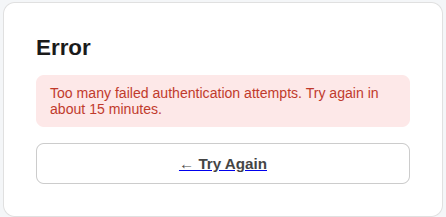
\includegraphics[width=0.9\columnwidth]{images/lockout}
  \caption{Account locked after five failed factor verifications.}
  \label{fig:lockout}
\end{figure}

\subsection{Encrypted TOTP Secrets at Rest (B3)}
TOTP secrets are stored as
$\text{nonce}_{12} \,\|\, \text{ciphertext} \,\|\, \text{tag}_{16}$
under AES-256-GCM.
The 32-byte master key is loaded from \texttt{IAA\_MASTER\_KEY} and
validated at startup; if the variable is missing, empty, or contains a
placeholder value, the process exits with code~78.

\subsection{Peer Lease Expiry (B4)}
Every row in \texttt{wg\_peers} carries an \texttt{expires\_at} timestamp
(default 24\,h, configurable in \texttt{srvauthn.conf}).
A daemon thread in \texttt{server/leases.py} polls every 60 seconds, removes
expired peers from the \texttt{wg0} interface via \texttt{wg set wg0 peer
<pub> remove}, and marks the row inactive.
This limits how long a compromised or abandoned session remains active on
the gateway.

\subsection{FIDO2 User Verification Required (B5)}
Both the helpdesk registration and the login flow set
\texttt{user\_verification=REQUIRED} for all WebAuthn operations.
The library default is \texttt{PREFERRED}, which silently falls back to
presence-only verification; \texttt{REQUIRED} ensures a PIN or biometric
check is always performed regardless of device capability.
